\documentclass{article}
\usepackage[utf8]{inputenc}
\usepackage{geometry}
\usepackage{graphicx}
\usepackage{pgfplots}
\usepackage{amsmath}
\usepackage{amssymb}
\usepackage{amsfonts}
\usepackage{mdframed}
\usepackage{amsthm}
\usepackage{tikz}
\usepackage{multicol}
\usepackage{cancel}
\usepackage{hyperref}
\newcommand{\cls}{^{\circ}C}

\geometry{a4paper, left=2cm, right=2cm, top=1cm, bottom=2cm}

\pgfplotsset{compat=1.18}
\begin{document}

\begin{minipage}{0.7\textwidth}
    \small \textbf{Fenómenos Colectivos}  \\
    \small {Facultad de Ciencias, Universidad Nacional Autónoma de México} \\
    \small {Profesora: Dra. Catalina Elizabeth Stern Forgach} \\
    \small {Ayudante: M. Tyra Delgadillo Mendoza} \\
    \small {Fecha de entrega: Miércoles 24 de Abril del 2024} \\
    \small {Nombre completo: Andrés López González} \\
    \small {Tarea III}
\end{minipage}
\hfill
\begin{minipage}{0.12\textwidth}
    
\includegraphics[width=\linewidth]{logo_universidad}
\end{minipage}\\\\

I. Un recipiente cilíndrico de 50cm de altura y 5 cm de diámetro que está sobre el piso se llena de agua hasta el tope. Se perfora un orificio de 1 cm de diámetro a una profundidad de 35cm. Determina la velocidad de salida del de agua y la distancia a la que cae al suelo el chorro de agua. \\
\textit{Considérese la ecuación de Torriceli.}\\
\begin{equation}
    v = \sqrt{2g \Delta y}
\end{equation}
\textit{Sustituimos.}
\begin{equation*}
    v_Q = \sqrt{2 \cdot 9.8066\frac{m}{s^2} \cdot (0.5m-0.35m)} \approx 1.7152 \frac{m}{s}
\end{equation*}
\textit{Para la distancia que cae utilizamos la ecuación más básica de la cinemática asumiendo que el comportamiento de una partícula fluída será el mismo para todas las demás.}
\begin{equation}
    \Vec{r}=\Vec{r_0} + \Vec{v_0}t + \frac{1}{2}\Vec{a}t^2
\end{equation}
\textit{Fijamos nuestro origen en $\Vec{r_0}$ de modo que coincide con la posición del agujero, vemos que la velocidad inicial es la horizontal por la cual sale el fluido y nuestra única aceleración es la gravitacional, además como está a 25cm del suelo sabemos que el tiempo que caerá en caer se determina por una simple caída libre de la forma $t=\sqrt{\frac{2y}{g}}$ por lo que sustituimos.}
\begin{align*}
    \Vec{r} &= \Vec{0} + (v_Q, 0 \frac{m}{s})\sqrt{\frac{2y}{g}} + \frac{1}{2}(0 \frac{m}{s^2},g)\cdot\frac{2y}{g} \\
    &= (\sqrt{2 \cdot 9.8066\frac{m}{s^2} \cdot (0.15m) }\cdot \sqrt{\frac{2(0.15)}{9.8066}}s, 0 \frac{m}{s}s) + (0m,0.15) \\
    &= (0.3m,0m) + (0m,0.15m) \\
    &= (0.3m,0.15m)
\end{align*}
\textit{Véase que esto tiene todo el sentido pues evidentemente en y solo le queda bajar la distancia del agujero al suelo (15cm) mientras que en x con un poco de álgebra llegamos a algo de la forma $\sqrt{2\cdot 0.15m}\sqrt{2\cdot 0.15m}=0.3m=30cm$, obtenemos la norma del vector posición final de la partida fluida para ver qué distancia recorrió $\sqrt{30^2+15^2}cm=15\sqrt{5}cm\approx 33.54101cm$}\\\\
II. Considera una serie de líneas de corriente en un canal. \\
a. Si el canal es recto, ¿cómo cambia la presión en la dirección perpendicular al flujo? \\
\textit{En un canal recto, donde el flujo es paralelo a las paredes del canal y el canal tiene un ancho constante, la presión a través del canal tiende a ser uniforme en la dirección perpendicular al flujo. Esto se debe a que el flujo sigue líneas paralelas sin obstáculos ni cambios en la geometría del canal. No se espera que haya gradientes significativos de presión en la dirección perpendicular, siempre y cuando el flujo sea laminar o turbulento pero estable, y no haya efectos como paredes rugosas o cambios bruscos en la sección transversal.}\\
b. Si el canal se curva, ¿cómo cambia la presión en la dirección perpendicular al flujo? \\
\textit{En un canal curvo, la presión cambia en la dirección perpendicular al flujo debido a la fuerza centrípeta necesaria para mantener el flujo en una trayectoria curvada. El fluido en un canal curvo experimenta una aceleración hacia el centro de la curvatura, lo que genera un gradiente de presión. La presión es mayor en el lado externo de la curva y menor en el lado interno, lo que se conoce como efecto de presión radial. Este gradiente de presión es necesario para mantener el flujo en la curva y es más pronunciado cuanto más cerrada es la curva o cuanto mayor es la velocidad del flujo.}\\
c. ¿Crees que después de la curvatura el flujo sea más complicado que antes de la curvatura? \\
\textit{Sí, después de una curva, el flujo puede ser más complicado. La curvatura induce gradientes de presión y fuerzas centrípetas que pueden llevar a la separación del flujo, turbulencia y formación de remolinos. El cambio en la dirección del flujo puede crear regiones de alta y baja presión, aumentando la complejidad del patrón de flujo. El efecto del cambio en la dirección del flujo también puede causar fluctuaciones en la velocidad, conduciendo a una mayor inestabilidad y variabilidad en el comportamiento del fluido.}\\\\
\begin{figure}[h]
    \centering
    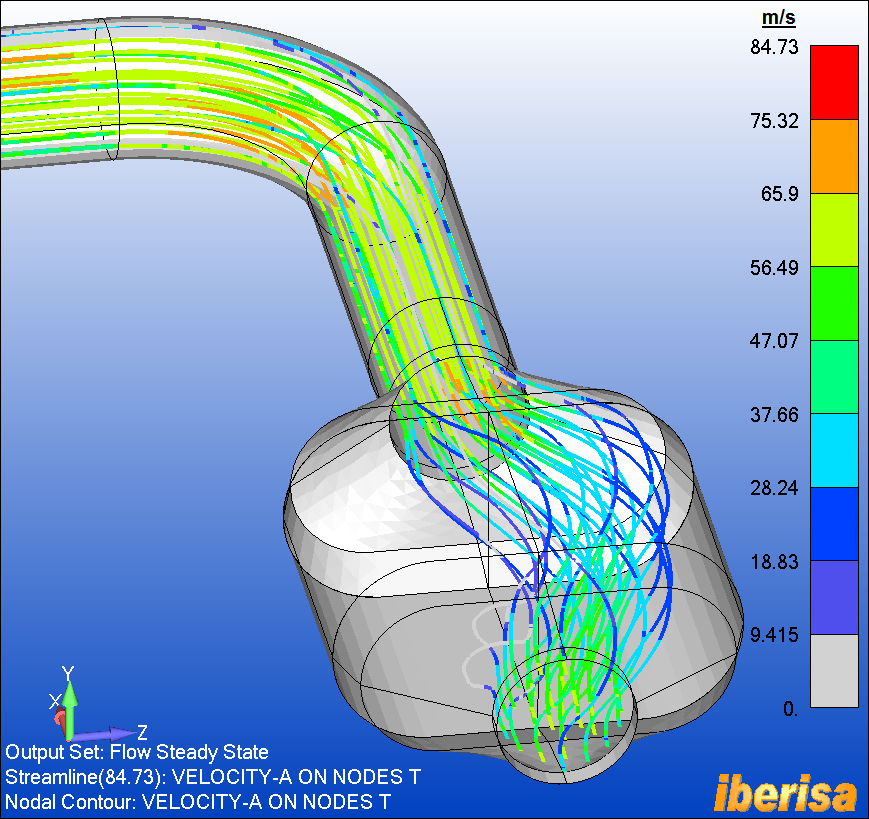
\includegraphics[width=0.5\linewidth]{hidrodynamics.png}
    \caption{Hidrodinámica.}
    \label{fig:enter-label}
\end{figure}\\\\
III. Explica cómo funcionan un tubo de Pitot y un tubo de Venturi.\\
\textit{Un tubo de Pitot es un dispositivo utilizado para medir la velocidad del fluido o la velocidad del aire en un entorno como en aeronáutica o sistemas de tuberías. Consiste en un tubo con una abertura en la parte delantera que apunta directamente al flujo. El tubo mide la presión total (suma de presión estática y dinámica) cuando el fluido entra y se detiene en el tubo. También tiene aberturas laterales para medir la presión estática (presión debido al fluido en reposo o flujo sin movimiento). La diferencia entre la presión total y la presión estática da la presión dinámica, que se puede usar para calcular la velocidad del flujo utilizando la ecuación de Bernoulli.}\\
\textit{Un tubo de Venturi en cambio es un dispositivo utilizado para medir el caudal de un fluido en un sistema de tuberías o para crear un área de baja presión para procesos como aspiración o mezcla de gases. El tubo tiene una sección estrecha en el centro y dos extremos más anchos. Cuando el fluido fluye a través de la sección estrecha, su velocidad aumenta debido a la conservación de la masa, lo que reduce la presión según nuevamente la ecuación de Bernoulli. Al medir la presión antes y después de la sección estrecha, se puede calcular la velocidad y el caudal del fluido. Este principio se utiliza en aplicaciones industriales para medir flujo o crear zonas de baja presión para aspiración o succión.}
\\\\
IV. Un tubo en U funciona como un sifón. La curvatura (A) está 1m por encima de la superficie de agua. La salida del tubo está 7 m por debajo de la superficie de agua. El agua sale del tubo del sifón a presión atmosférica, determina la velocidad de salida y la presión absoluta del agua en la curvatura (A). Lista las hipótesis que haces para poder resolver este problema.\\
\begin{figure}[h]
    \centering
    
\includegraphics[width=0.2\linewidth]{image.png}
    \caption{Problema IV}
    \label{fig:enter-label}
\end{figure}\\
\textit{Considérese la ecuación de Bernoulli.}
\begin{equation}
    P_1 + \frac{1}{2}\rho v_1^2 + \rho gz_1 = P_2 + \frac{1}{2}\rho v_2^2 + \rho gz_2
\end{equation}
\textit{Véase que la presión independiente en ambos casos es la atmosférica y la velocidad 1 evidentemente es cero, asímismo se indica que $z_1=0m$, finalmente obsérvese que $z_2=-8m+1m=-7m$. Simplificamos obteniendo la siguiente ecuación.}
\begin{align*}
    0 &= \frac{1}{2}\rho v_2^2 + \rho gz_2 \\
      &= \frac{1}{2}v_2^2 + gz_2 \\
    -2gz_2 &= v_2^2 \\
    \sqrt{-2gz_2} &= v_2 \\
    \sqrt{2(9.8066\frac{m}{s^2})7m} &= \\
    11.71718 \frac{m}{s} &\approx
\end{align*}
\textit{Ahora para la presión absoluta del agua en la curvatura (A) usamos nuevamente la ecuación de Bernoulli.}
\begin{align*}
    P_1 + \frac{1}{2}\rho v_1^2 + \rho gz_1 &= P_A + \frac{1}{2}\rho v_A^2 + \rho gz_A \\
    P_1 &= \\
    P_A &= P_1 - (\frac{1}{2}\rho v_A^2 + \rho gz_A) \\
    &= P_atm - (\frac{1}{2}\rho v_A^2 + \rho gz_A)  \\
    &= 1.013\cdot10^5 Pa - (\frac{1}{2}(997\frac{kg}{m^3}) (11.71718 \frac{m}{s})^2 + (997\frac{kg}{m^3}) (9.8066\frac{m}{s^2})(1m)  \\
    &= 23,082.60468 Pa
\end{align*}
\end{document}